%! suppress = MissingImport
%! suppress = UnresolvedReference


\section{Background and Previous System} \label{sec:background-and-previous-system}
This chapter establishes the educational and technical baseline for the thesis.
It first motivates the educational relevance of Linux command-line practice in a web-based environment and situates the work within two earlier iterations of the learning environment developed at the University of Tartu.
It then outlines the architecture and Azure deployment model of the previous system and identifies the main unresolved limitations that define the modernization context for this work.

\begin{figure}[H]
  \centering
  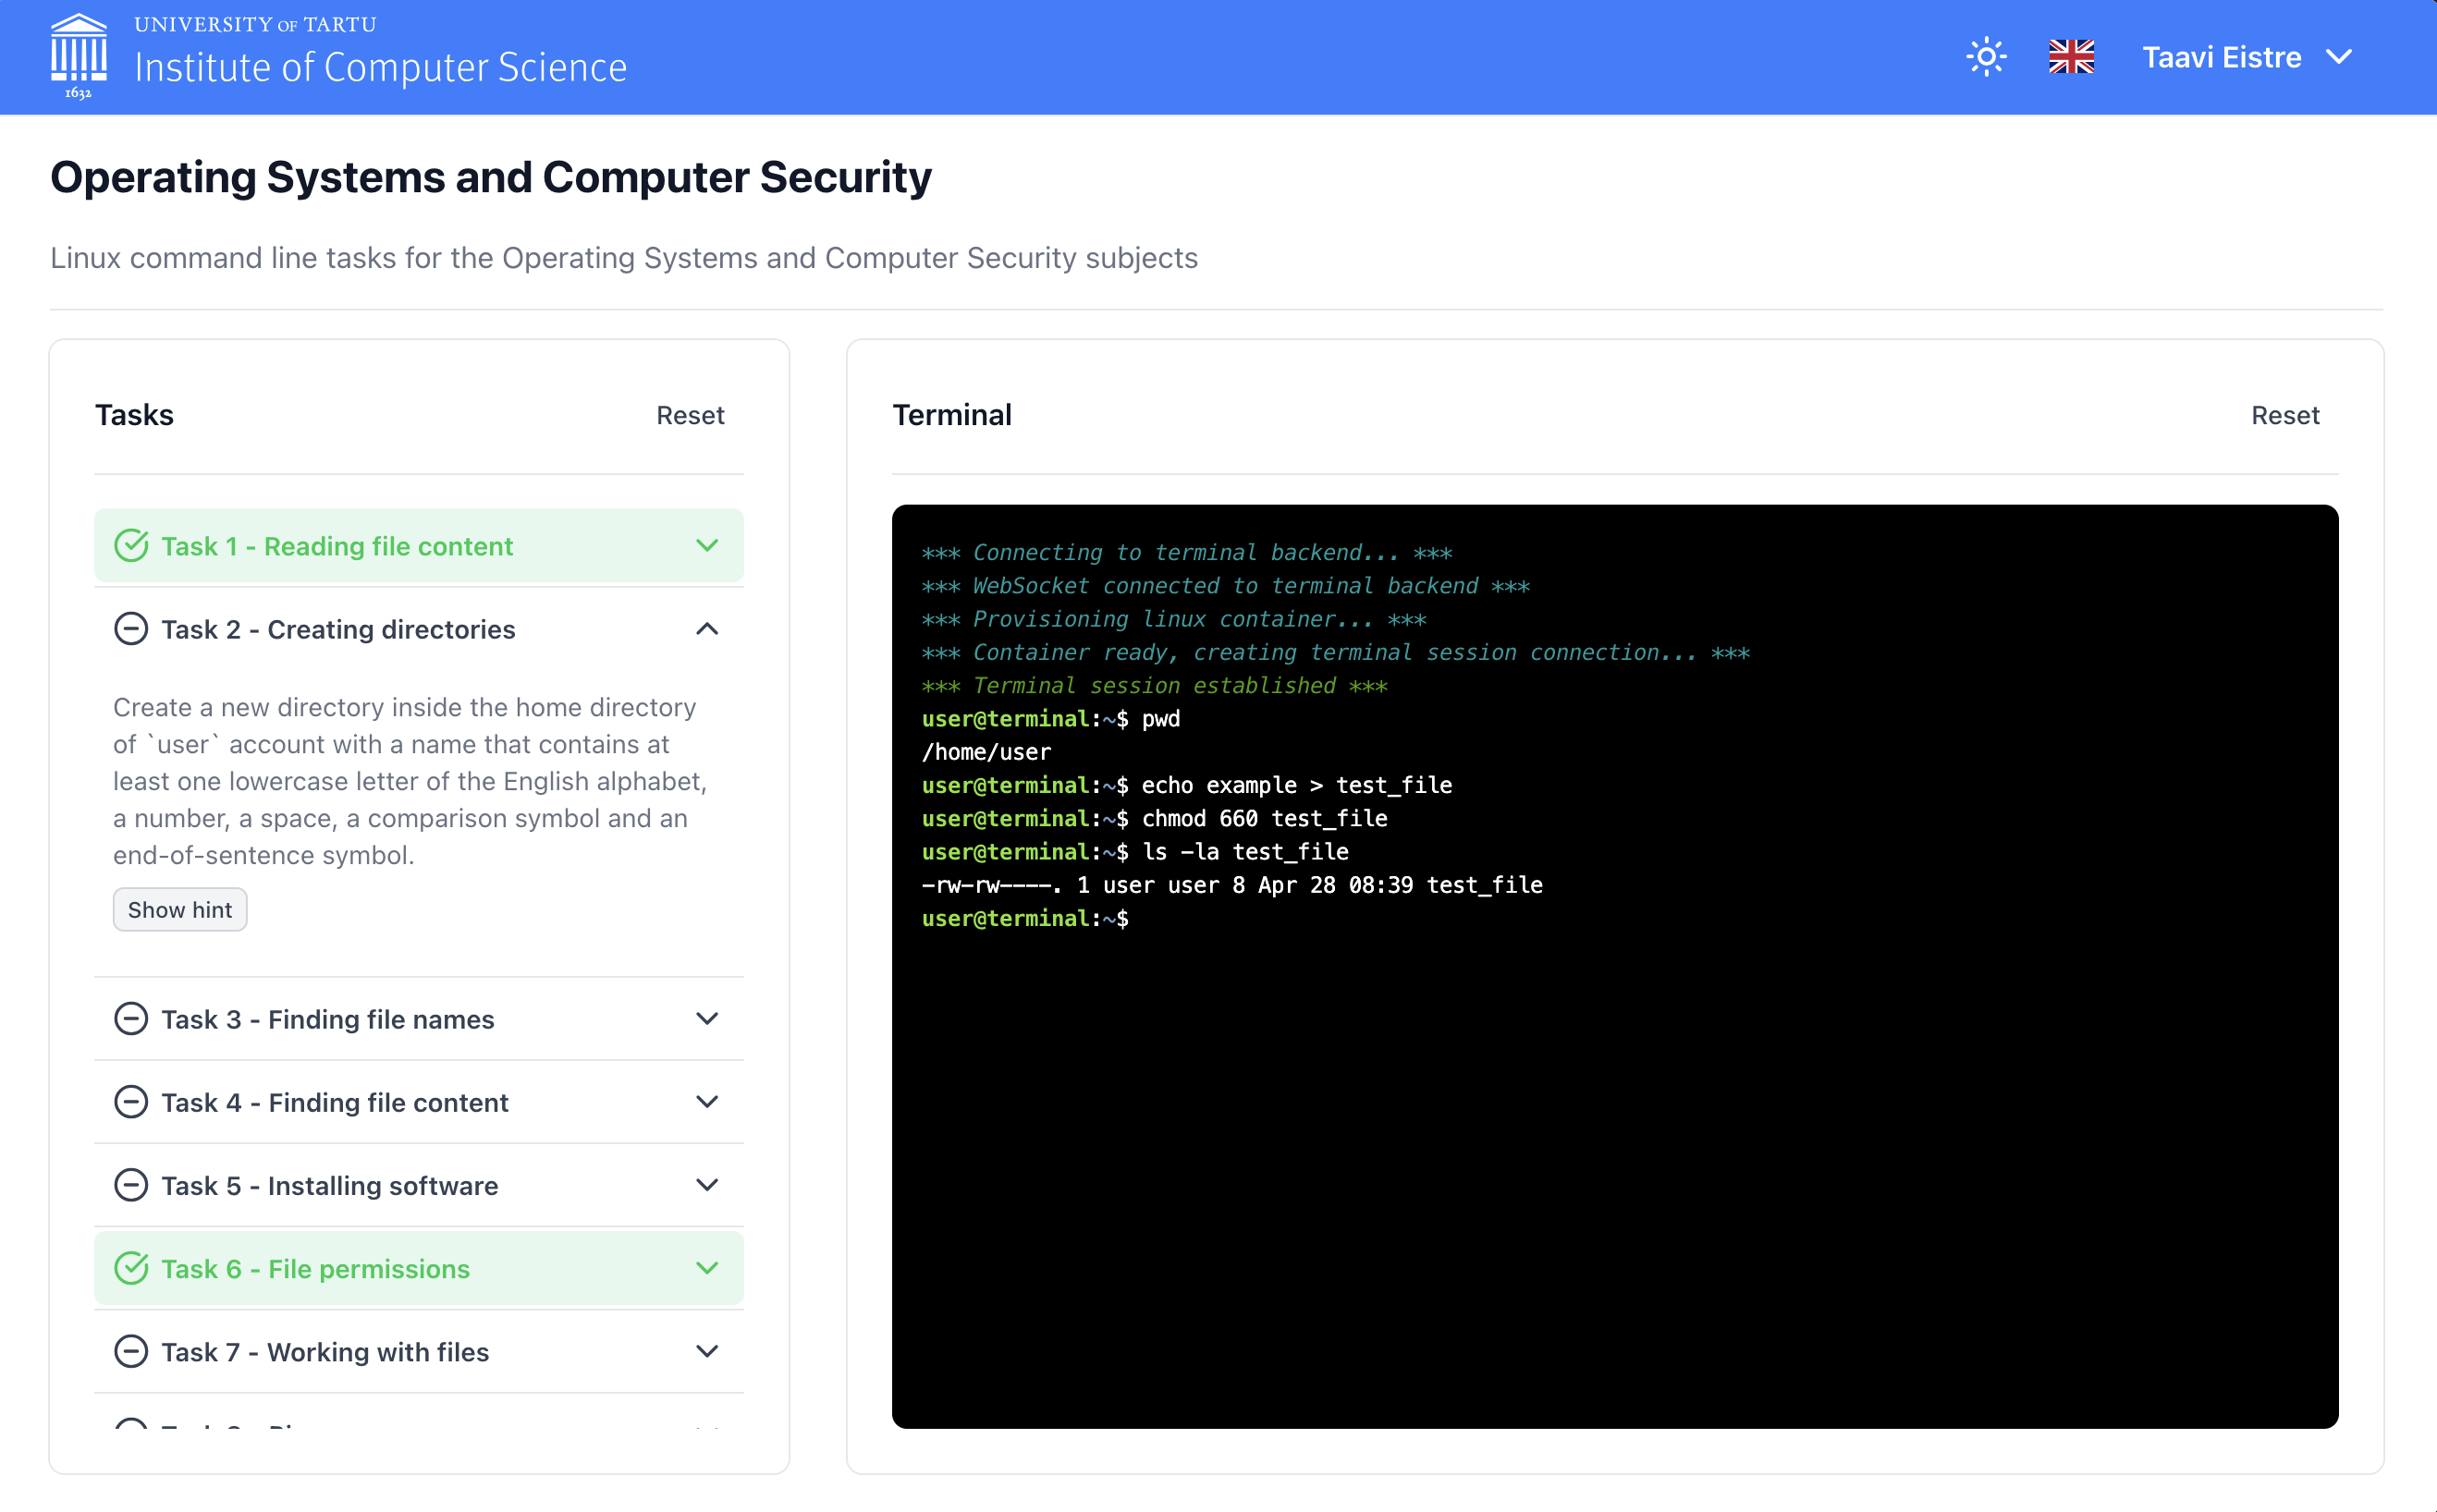
\includegraphics[width=\textwidth]{figures/figure1-environment}
  \caption{User-facing view of the revised web-based Linux command-line learning environment.}
  \label{fig:updated-learning-environment}
\end{figure}

For orientation, Figure~\ref{fig:updated-learning-environment} shows the revised learning environment with its task list, task status indicators, and browser-based Linux terminal.

\subsection{Motivation and Prior Work} \label{subsec:motivation-and-prior-work}
Linux command-line knowledge remains important in many systems-oriented computing roles, including system administration, software development, and automation.
Because Linux environments are often administered through terminal-centric workflows, hands-on command-line practice remains a relevant educational objective.
This view is also reflected in prior academic literature.
Švábenský et al.~\cite{svabensky_toolset_2021} characterize the Linux command-line interface as common in higher education and software development contexts and argue that studying command-line interactions can support hands-on learning.
Similarly, Bailey and Zilles~\cite{bailey_uassign_2019} treat terminal skills as suitable for interactive, auto-graded assessment through authentic terminal actions.
At the University of Tartu, command-line work is especially relevant in courses such as ``Operating Systems'' (LTAT.06.001) and ``Computer Security'' (LTAT.06.002).

Earlier thesis work at the University of Tartu developed the learning environment in two main iterations.
Halapuu's proof-of-concept implementation~\cite{halapuu_2022} introduced the first iteration of the web-based environment, providing each student with a browser-based terminal connected to an isolated Linux environment and supporting automatic task checking based on observable outcomes such as command output and filesystem changes.
It was tested in the ``Computer Security'' course with over one hundred participants, demonstrating that the approach was viable in a practical course setting~\cite{halapuu_2022}.
However, its deployment on the supervisor's university laptop left stability, security, and maintainability concerns unresolved.

Eistre's bachelor's thesis~\cite{eistre_2024} transformed the prototype into a cloud-hosted learning platform intended for sustained use.
That version improved the system architecture, added bilingual support, and replaced the earlier local deployment model with a cloud-hosted one.
It was evaluated in the ``Computer Security'' course in February 2024 with 382 participants~\cite{eistre_2024}.
The system was successful overall, but later use exposed limitations in maintainability, deployment reproducibility, portability, and cost efficiency.
This thesis builds on that baseline by addressing these limitations while preserving the established educational workflow.

\subsection{Architecture and Deployment of the Previous System} \label{subsec:architecture-and-deployment-of-the-previous-system}
This section outlines the system developed in Eistre's thesis~\cite{eistre_2024}, which serves as the technical starting point for this master's thesis.
The focus is on the application's internal architecture and Azure-based deployment model because both directly shape the cost, maintainability, and operational constraints that later chapters address.

\subsubsection{System Architecture} \label{subsubsec:system-architecture}
The previous system was designed as a production-oriented web-based Linux command-line learning environment for cloud deployment and sustained use~\cite{eistre_2024}.
Its implementation used TypeScript\footnote{\url{https://www.typescriptlang.org/}}, Node.js\footnote{\url{https://nodejs.org/}}, and the Nuxt 3 framework\footnote{\url{https://nuxt.com/}} for both the user interface and server-side logic.
Figure~\ref{fig:baseline-system-architecture} illustrates the system's main components and the runtime interactions between them.

\begin{figure}[H]
  \centering
  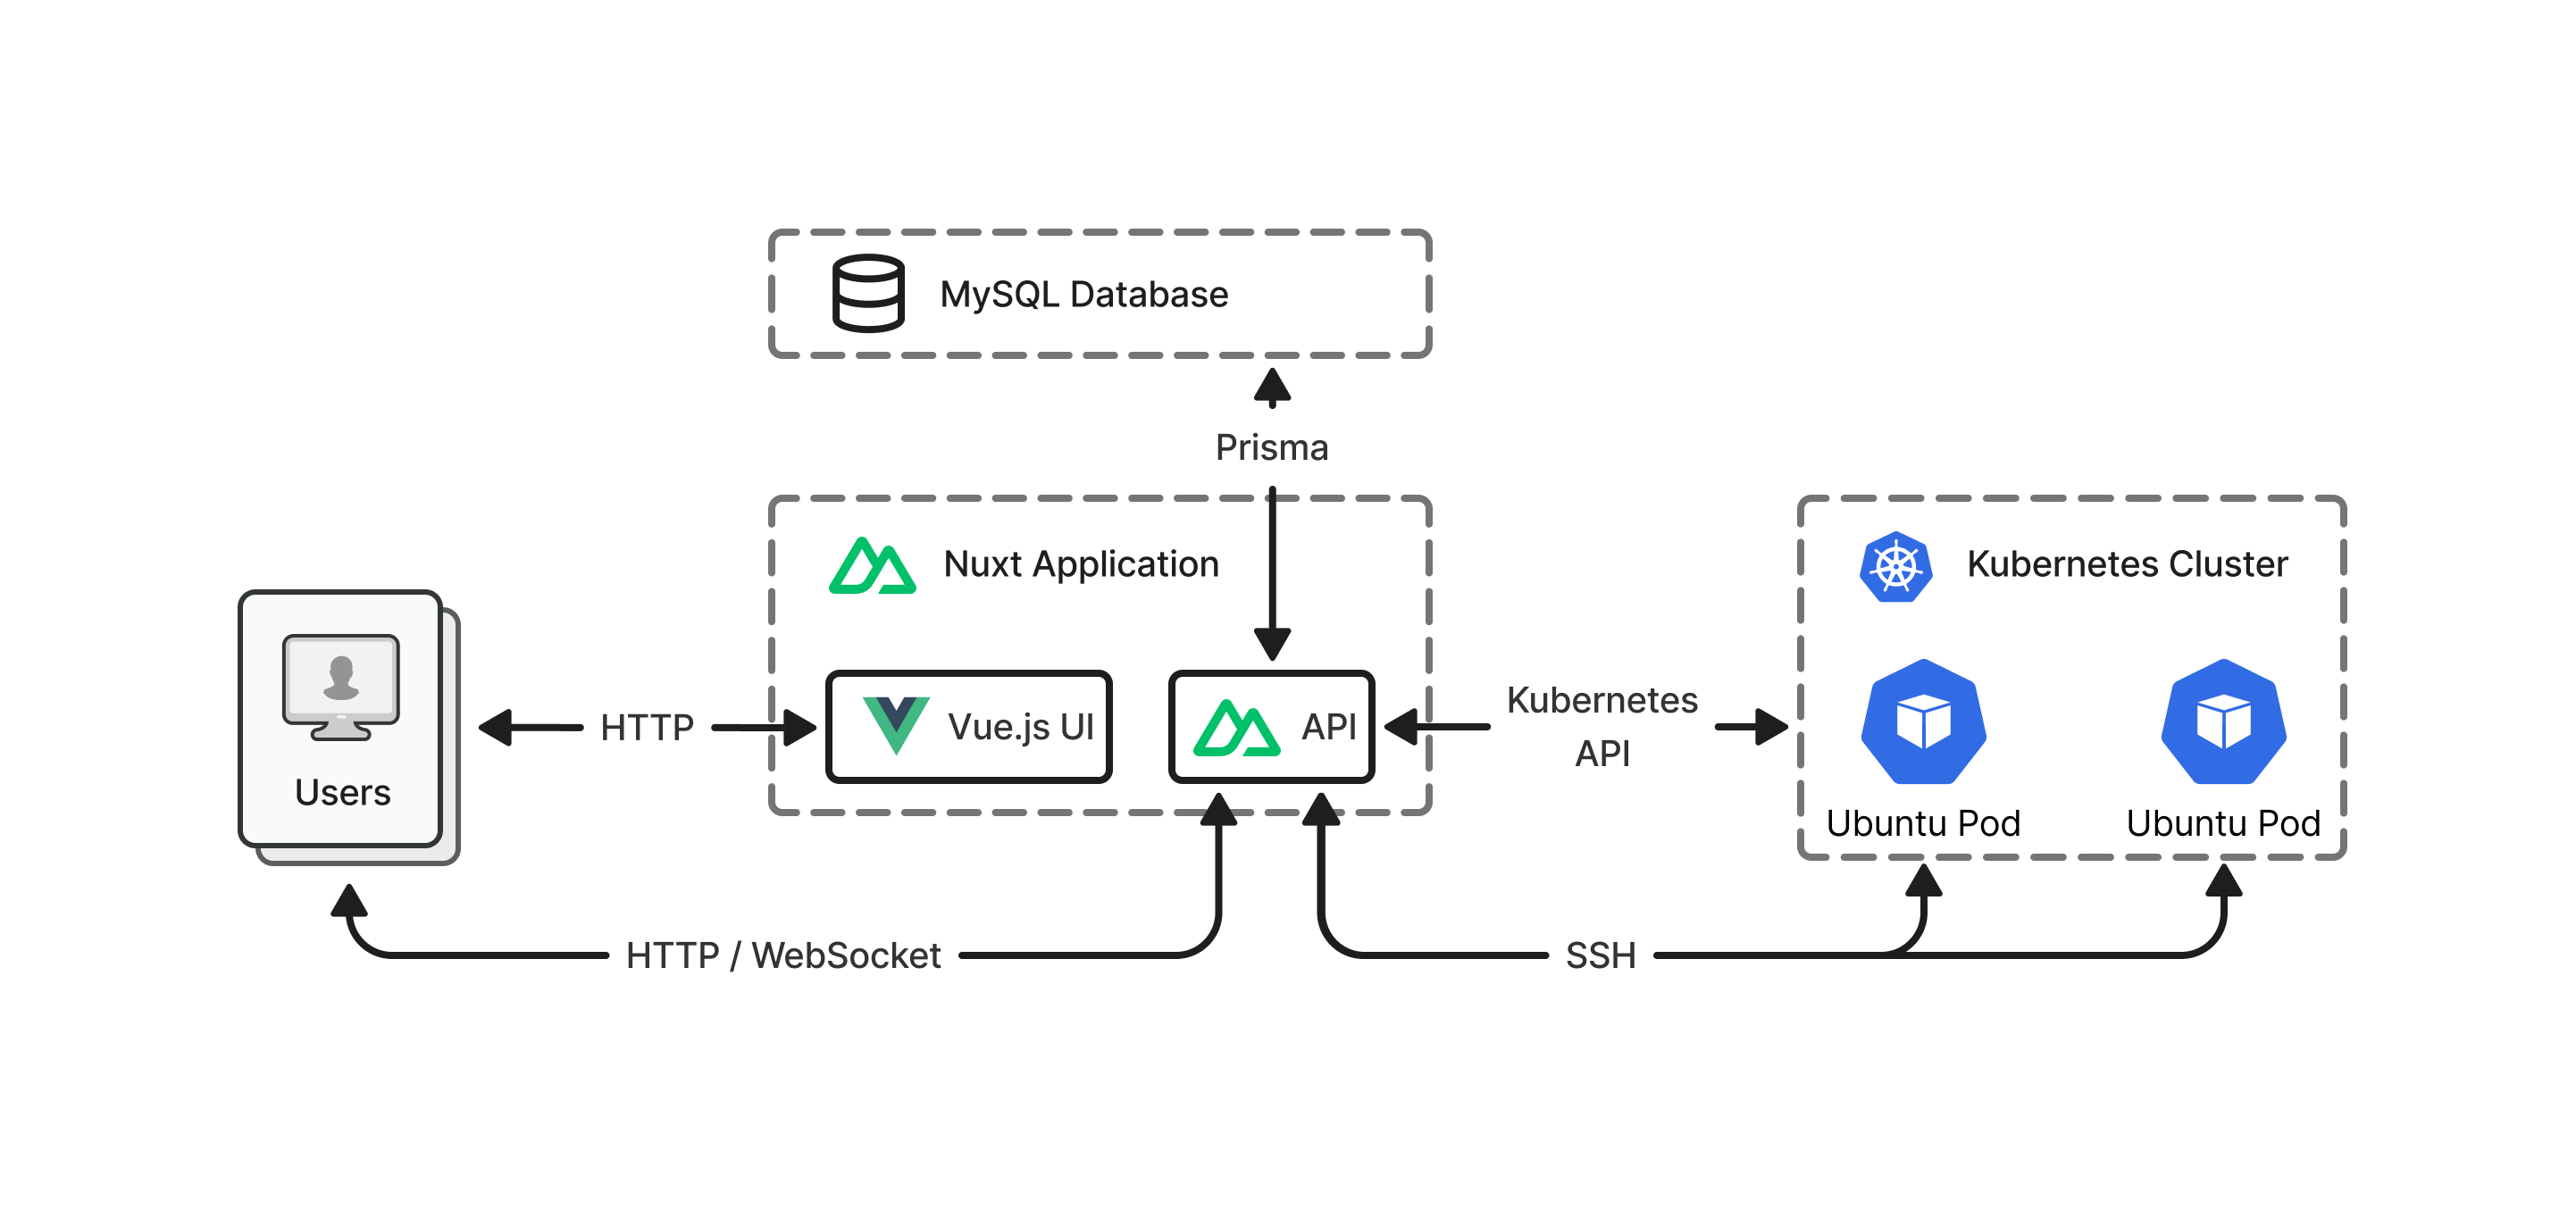
\includegraphics[width=\textwidth]{figures/figure2-baseline-architecture}
  \caption{Baseline system architecture of Eistre's implementation, adapted from~\cite{eistre_2024}.}
  \label{fig:baseline-system-architecture}
\end{figure}

The architecture is organized around four main components.
These are a client-side user interface, a server-side backend API (application programming interface), a MySQL\footnote{\url{https://www.mysql.com/}} database, and a Kubernetes\footnote{\url{https://kubernetes.io/}} cluster that provisions isolated Linux environments~\cite{eistre_2024}.
At runtime, the browser-based terminal communicates with the API layer, which brokers interaction with a user-specific Linux container in Kubernetes and records user accounts, learning content, and progress in MySQL\@.
The client-side interface, implemented with Vue.js\footnote{\url{https://vuejs.org/}} and Nuxt, supports account registration and authentication, topic navigation, task solving, administrative content management, and usage in both English and Estonian.
The server-side application acts as the coordination layer by managing sessions, provisioning and cleaning up per-user Linux environments, bridging terminal traffic, checking task completion conditions, and recording progress.

At an architectural level, the previous system already satisfied the core functional requirements of the learning environment.
For that reason, this thesis treats it as a system to be modernized and refined rather than replaced in its entirety.

\subsubsection{Cloud Deployment on Azure} \label{subsubsec:cloud-deployment-on-azure}
The previous system was deployed on Microsoft Azure~\cite{eistre_2024}.
Azure was chosen in part because it offers educational credits to students, which made it a practical option for an academic project.
The application was containerized and deployed using Azure Container Apps\footnote{\url{https://azure.microsoft.com/en-us/products/container-apps}} (ACA) for the web application and Azure Kubernetes Service\footnote{\url{https://azure.microsoft.com/en-us/products/kubernetes-service}} (AKS) for per-user Linux environments~\cite{eistre_2024}.
Figure~\ref{fig:azure-deployment-overview} provides a deployment-level overview of the baseline environment and the Azure services created for it.

\begin{figure}[H]
  \centering
  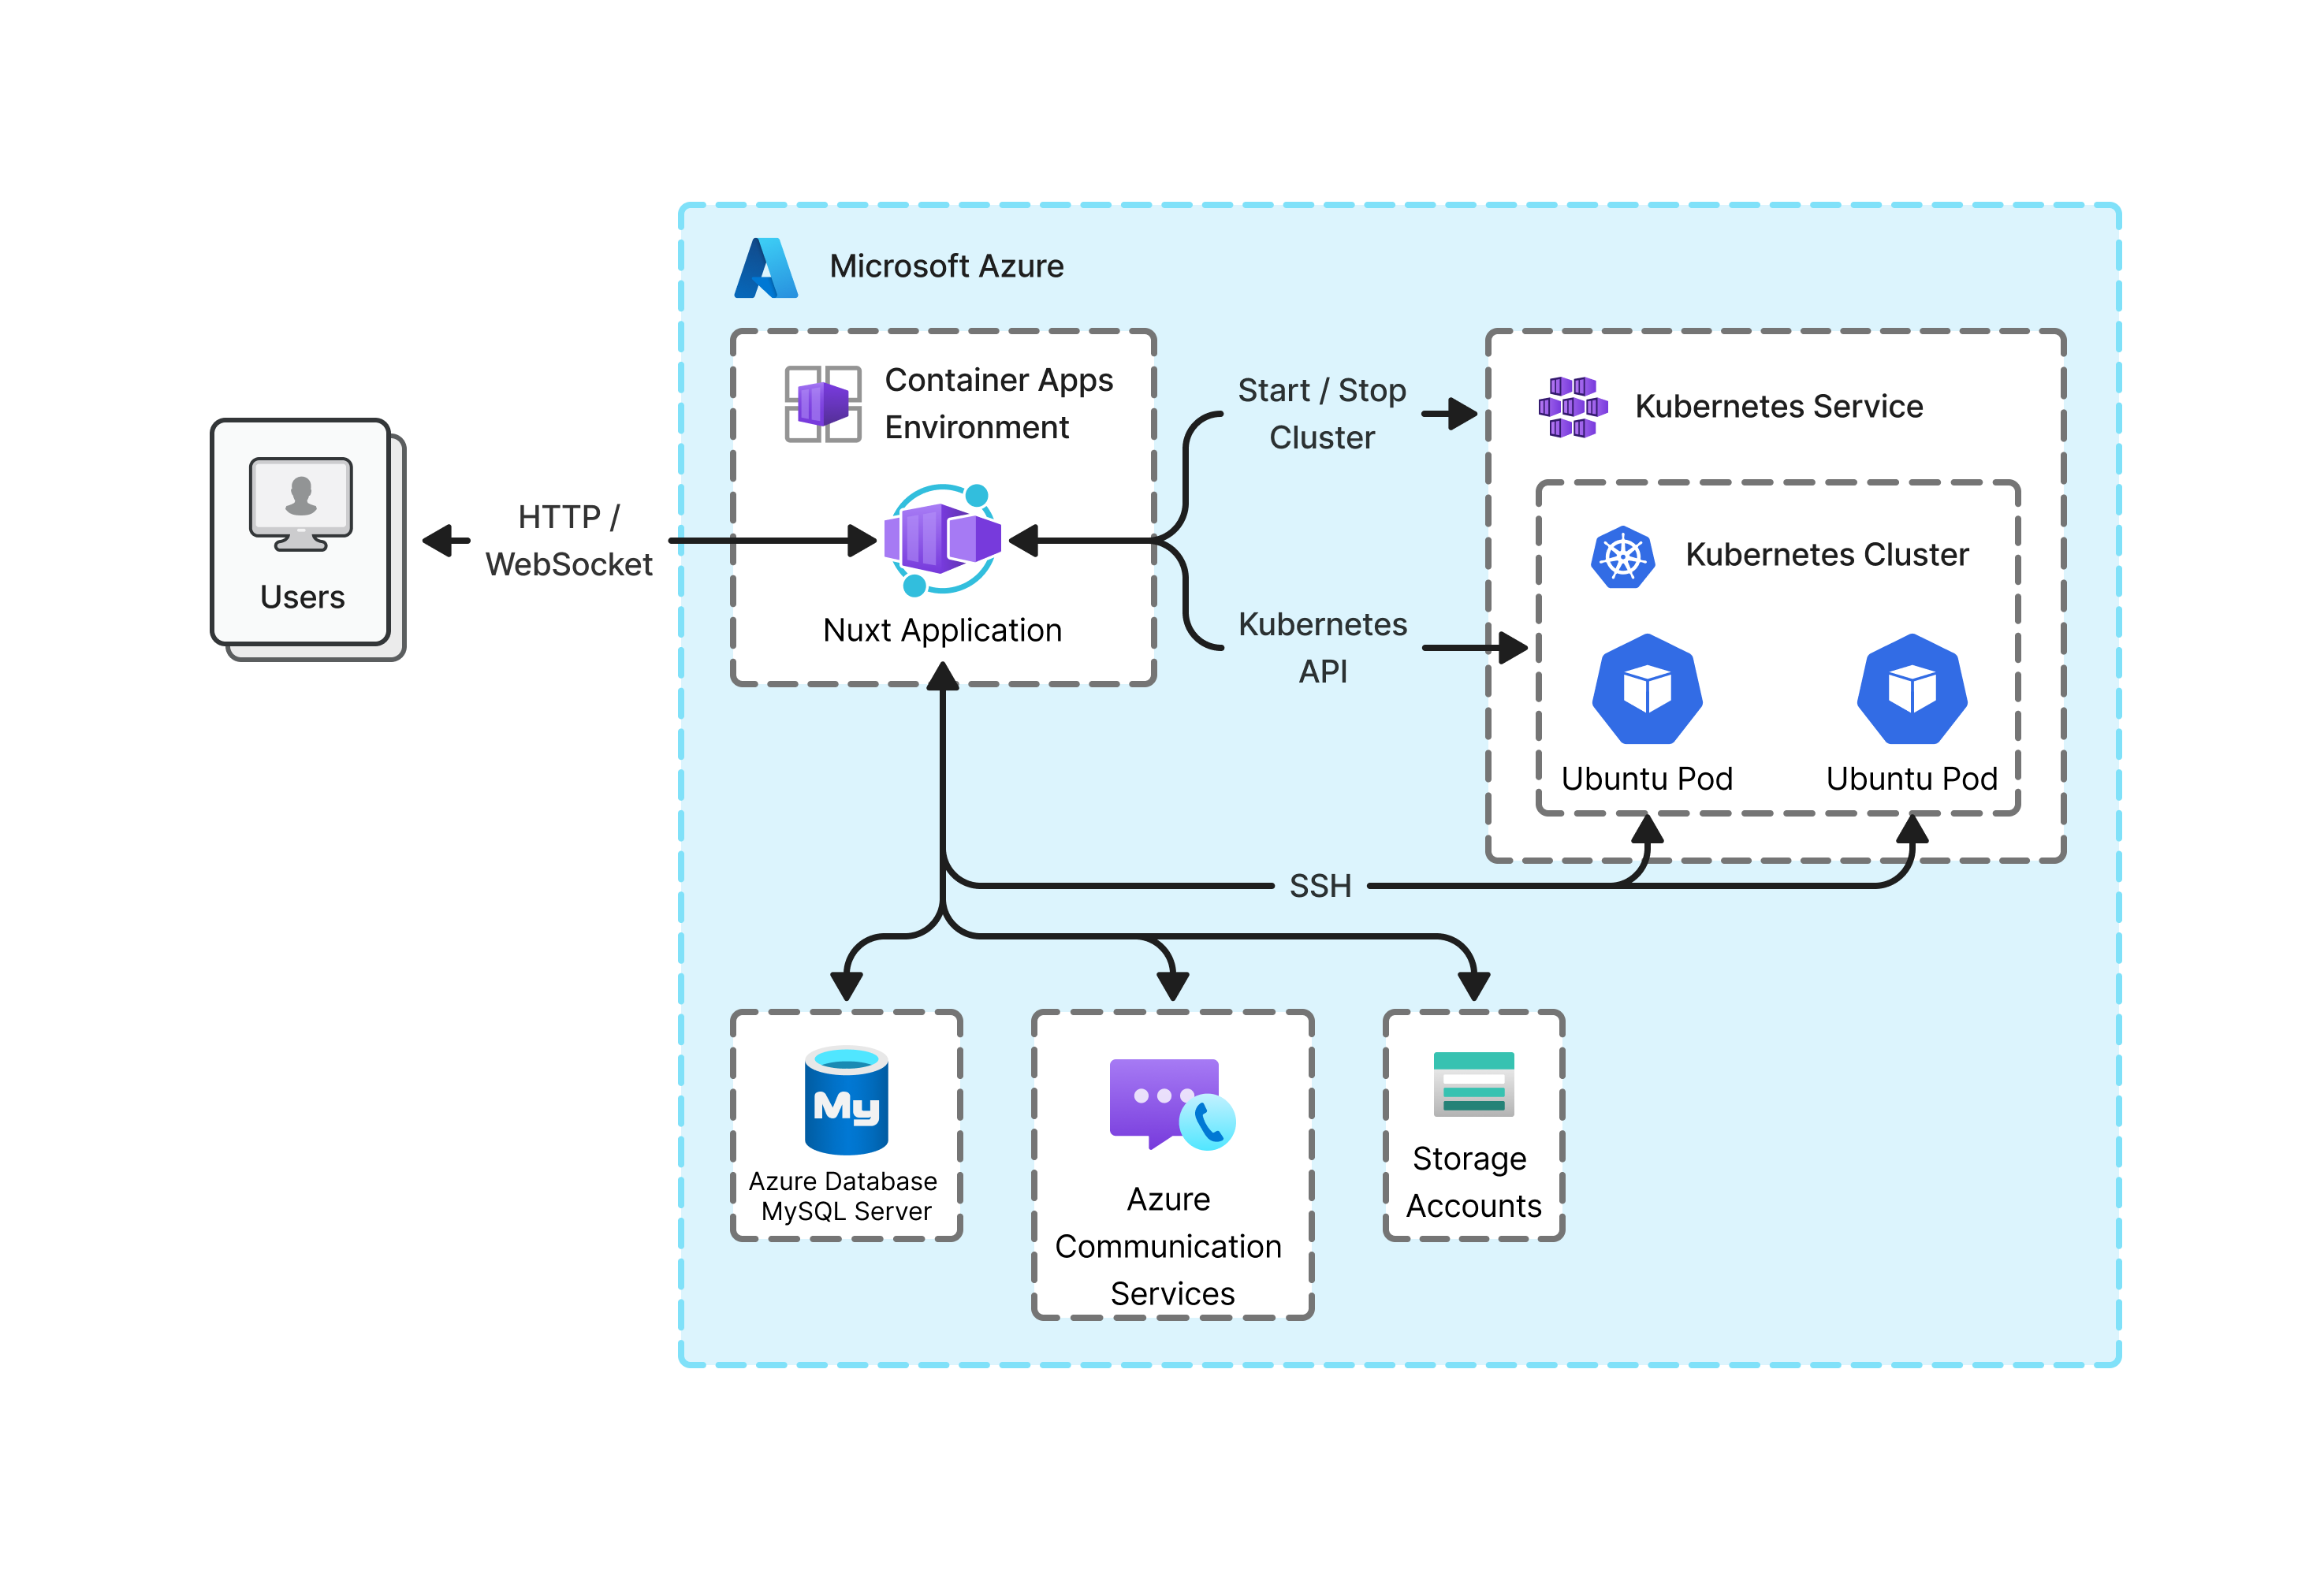
\includegraphics[width=\textwidth]{figures/figure3-baseline-azure}
  \caption{Azure deployment overview of Eistre's baseline system, adapted from~\cite{eistre_2024}.}
  \label{fig:azure-deployment-overview}
\end{figure}

In this design, the Nuxt application ran as a single ACA instance with fixed resource reservations of 0.5 vCPU and 1 GB of memory~\cite{eistre_2024}.
Interactive Linux sessions were provisioned in an AKS cluster configured with B2s virtual machines~\cite{eistre_2024}.
Because a continuously running Kubernetes cluster can create a significant baseline cost even without active course usage, the system included start and stop logic for the AKS cluster~\cite{eistre_2024}.
When a user initiated a session while the cluster was stopped, the environment started the cluster and showed a waiting state.
After an idle period, the cluster could be stopped again to reduce unused compute cost.

In addition to compute and container orchestration, the deployment relied on several supporting Azure services~\cite{eistre_2024}.
These included Azure Communication Services\footnote{\url{https://azure.microsoft.com/en-us/products/communication-services}} for email delivery, Azure Files\footnote{\url{https://azure.microsoft.com/en-us/products/storage/files}} for key storage, and Azure Database for MySQL\footnote{\url{https://azure.microsoft.com/en-us/products/mysql}} for persistent application data~\cite{eistre_2024}.
This model established a functional cloud-based operating environment, but it also introduced the cost and operational profile that became central to the modernization and cost-optimization goals of this thesis.

\subsection{Limitations and Improvement Opportunities} \label{subsec:limitations-and-improvement-opportunities}

While the cloud-enabled learning platform developed in Eistre's bachelor's thesis~\cite{eistre_2024} represented a significant advance over the initial prototype, it also exposed several limitations and challenges.
This section summarizes the key issues in the baseline system and clarifies why they matter for the modernization and cost-optimization work described in later chapters.

\subsubsection{Cost Structure} \label{subsubsec:cost-structure}
A significant limitation of the baseline system was its cost structure in the cloud-hosted environment.
Table~\ref{tab:baseline-azure-costs} summarizes two observed monthly cost breakdowns from the previous Azure deployment during July 2025, a minimal-usage month, and September 2025, an active-semester month.
The corresponding billing screenshots are provided in Appendix~\ref{app:azure-cost-evidence}.

\begin{table}[H]
  \centering
  \caption{Observed cost structure of the baseline Azure deployment.}
  \label{tab:baseline-azure-costs}
  \begin{tblr}{
    width=1.0\textwidth,
    hlines,
    vlines,
    colspec = {Q[l,font=\bfseries] Q[c] X[l]},
    row{1} = {font=\bfseries},
  }
    Period & Total cost & Main cost drivers \\
    July 2025 & €52.88 & Azure Database for MySQL (€26.90), Load Balancer (€13.62), Azure Container Apps (€8.92) \\
    September 2025 & €93.12 & Same components as for July, AKS virtual machine compute (€18.45) and its supporting services \\
  \end{tblr}
\end{table}

Taken together, these observations show that the main issue was not simply that cloud infrastructure incurred costs, but that the operational model of the previous deployment remained poorly matched to intermittent educational workloads.
Although the system already implemented demand-based cluster start and stop mechanisms, idle costs remained significant and active periods still generated significant compute and supporting service charges.
This cost profile therefore defines the central optimization problem addressed in this thesis.
The task is to reduce the platform's always-on footprint while preserving per-user interactive Linux environments for irregular classroom usage.

\subsubsection{Deprecated Authentication Library} \label{subsubsec:deprecated-authentication-library}
The previous version of the learning environment relied on the Lucia\footnote{\url{https://github.com/lucia-auth/lucia}} authentication library to implement core authentication functionality, including user registration, login, and session management~\cite{eistre_2024}.
According to the Lucia maintainer, the project would be deprecated by March 2025 and would transition away from being a maintained, general-purpose authentication library~\cite{pilcrowonpaper_fresh_start_2024}.
By March 2025, Lucia had been repositioned primarily as an educational resource for learning about authentication implementation rather than as a long-term dependency for production systems~\cite{pilcrowonpaper_fresh_start_2024}.
Continued dependence on an unsupported authentication library would therefore increase authentication-related maintenance and security risk.
As a result, the authentication layer became a necessary modernization target, although the baseline requirements for user verification and session management remained unchanged.

\subsubsection{Outdated Dependencies} \label{subsubsec:outdated-dependencies}
A further limitation of the baseline system was its reliance on dependencies that inevitably become outdated over time, creating both maintainability and security risks.
Lauinger et al.~\cite{lauinger_thou_2017} show that delayed library updates are common in web ecosystems, finding that many websites use JavaScript libraries with known vulnerabilities and that outdated versions may remain in use for years.
Pashchenko et al.~\cite{pashchenko_qualitative_2020} further report that dependency update decisions often involve trade-offs between security, compatibility, and engineering effort.
The baseline system was developed using Nuxt 3~\cite{eistre_2024}, while Nuxt 4 has since become the current major release line~\cite{nuxt_roadmap}.
In addition to lifecycle considerations, older framework versions may also contain publicly disclosed vulnerabilities.
For instance, CVE-2025-27415 identifies a cache-poisoning issue affecting Nuxt versions prior to 3.16.0 in specific CDN (content delivery network) configurations~\cite{nvd_cve_2025_27415}.
Together, these points indicate that dependency modernization was a necessary part of maintaining the system's security posture and long-term compatibility.

\subsubsection{Additional Improvement Opportunities} \label{subsubsec:additional-improvement-opportunities}
In addition to the previously described cost and maintainability issues, the previous system exposed several further operational and usability limitations that are relevant to the later redesign.
First, the environment showed a scalability concern under classroom-scale load.
According to observations reported by the thesis supervisor, some students were at times unable to access an interactive shell session because the AKS node pool could not scale due to Azure quota constraints\footnote{Based on private communication with thesis supervisor Alo Peets.}.
This suggests that functional correctness alone was insufficient in practice and that the deployment also had to support classroom demand more reliably.
The issue therefore points to a reliability and scalability limitation relevant to the redesign.

Second, the content model did not natively support localization for topics and tasks.
Although the user interface supported multiple languages, equivalent learning content had to be duplicated for each locale, which increased maintenance overhead and created a risk of inconsistencies when content changed.
This arrangement indicates that the baseline content model was not well aligned with multilingual maintenance.
The issue therefore exposed a maintainability limitation in how localized learning content was represented.

Third, the authentication approach could be improved from a usability perspective by integrating the University's single sign-on capabilities.
Institutional login would simplify onboarding and align access control with existing university identity management, thereby improving the overall user experience.
In this case, the limitation concerns usability and institutional integration rather than core functionality.
Taken together, these observations identify additional redesign pressures related to reliability under classroom load, maintainability of multilingual content, and practical access management.

\subsubsection{Infrastructure as Code} \label{subsubsec:infrastructure-as-code}
An additional limitation of the baseline system was the high setup overhead needed to replicate the environment.
Deploying the environment required cloud knowledge and coordination of several prerequisites, such as managed database provisioning, container hosting configuration, and Kubernetes cluster setup.
In practice, reproducing the environment required manual setup across several cloud services and a comprehensive step-by-step deployment procedure that was difficult to reproduce consistently across environments.
This type of manual infrastructure configuration is widely recognized as slow and error-prone, especially as system complexity grows~\cite{guerriero_adoption_2019}.
Infrastructure as Code addresses this problem by representing infrastructure through reusable definition files, improving repeatability, and reducing configuration drift~\cite{guerriero_adoption_2019,bali_enhancing_2023}.
In this thesis, deployment automation is therefore relevant as a direct response to reproducibility and transferability problems in the baseline system.

Taken together, the previous system established a technically functional and educationally validated foundation for web-based Linux command-line learning.
However, the evidence presented in this chapter also indicates that its cloud deployment model remained suboptimal with respect to its cost profile, maintainability, deployment reproducibility, and some aspects of operational robustness.
These limitations define the modernization context of this thesis and provide the rationale for the redesign and implementation choices discussed in the following chapters.
